\section{Describe interaction of atoms with light by using the Einstein coefficients. Establish relationships between these coefficients. Relate the Einstein coefficients to spectroscopic experiments.}
\sectionmark{Atom-lysvekselvirkning og Einsteinkoefficienter}

\noindent
\large
Vi betragter atom-lysinteraktionen for et toniveausystem
\begin{itemize}
    \item 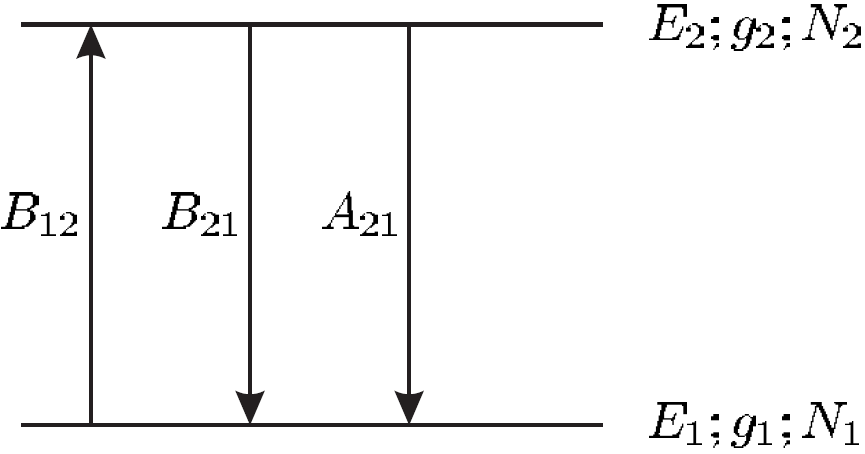
\includegraphics[width=0.6\textwidth]{Q02/images/TwoLevelSystem2.PNG}
    \item Grundtilstanden $\ket{1}$ og den exciterede tilstand $\ket{2}$ har henholdsvis energierne $E_1$ og $E_2$, udartetheden $g_1$ og $g_2$, og har en population på $N_1$ og $N_2$.
\end{itemize}
Sendes lys med energitæthed $\rho(\omega)$ ind på atomet, så vekselvirker atomet kun med den del, som har frekvens tæt på atomets resonansfrekvens $\omega_{12} = \Delta E / \hbar$. Vekselvirkningen kan føre til en af følgende ting:
\begin{itemize}
    \item Absorption af en foton med atomets resonansfrekvens kan excitere en elektron fra $\ket{1}$ til $\ket{2}$.
    \item Stimuleret emission af en foton med atomets resonansfrekvens samt at en elektron falder fra $\ket{2}$ til $\ket{1}$. Kommer af et symmetriargument.
\end{itemize}
Deruover kan det også forekomme spontan emission, hvor en foton med atomets resonensfrekvens udsendes, samt at en elektron falder fra $\ket{2}$ til $\ket{1}$. Dette sker \emph{uden} vekselvirkning med lys.\\\\
%
Ser vi på ændringen af populationen i energiniveauerne, så får vi rateligninger
\begin{align*}
    \frac{\text{d}N_2}{\text{d}t} &= N_1 B_{12} \rho(\omega_{12}) - N_2 B_{21} \rho(\omega_{12}) - N_2 A_{21} \: , \quad \text{og} \\
    \frac{\text{d}N_1}{\text{d}t} &= - \frac{\text{d}N_2}{\text{d}t} \: .
\end{align*}
Idet at der intet lys indsendes mod atomet ($\rho(\omega) = 0$) fås en eksponentielt aftagende løsning
\begin{align*}
    N_2(t) &= N_2(0)\exp(-A_{21}t) = N_2(0)\exp\left(-\frac{t}{\tau}\right) \: ,
\end{align*}
hvor $\tau^{-1}$ er den gennemsnitlige levetid af det exciterede niveau.\\\\
%
Sammenhængen mellem Einsteinkoefficienterne findes ved at placere toniveausystemet i et område af sorlegemetråling.
\begin{itemize}
    \item Energitætheden af lyset vil være givet ved Plancks lov
    \begin{align*}
        \rho(\omega) &= \frac{\hbar\omega}{\pi^2c^3} \dfrac{1}{\exp{\dfrac{\hbar\omega}{k_B T}} - 1} \: .
    \end{align*}
    \item Populationerne i atomet betragtes nu i ligevægt
    \begin{align*}
        0 &= \frac{\text{d} N_2}{\text{d} t} \quad \Rightarrow \quad \rho(\omega_{12}) = \frac{A_{21}}{B_{21}} \dfrac{1}{\dfrac{N_1 B_{12}}{N_2 N_{21}} - 1} \: .
    \end{align*}
    \item I termisk ligevægt vil hver af de udartede tilstande være givet ved Boltzmanfaktoren, hvor populationen i hver af disse udartede tilstande er totalpopulationen i energiniveauet uddelt på antallet af udartede tilstande i det, hvorfor vi får
    \begin{align*}
        \frac{N_2}{g_2} &= \frac{N_1}{g_1}\exp\left(-\frac{\hbar \omega}{k_B T}\right) \: .
    \end{align*}
\end{itemize}
Kombineres de ovenstående tre ligninger fås sammenhængen mellem Einsteinkoefficienterne
\begin{align*}
    A_{21} & =\frac{\hbar\omega^3}{\pi^2c^3} B_{21} \: , \quad \text{og} \quad B_{12} = \frac{g_2}{g_1} B_{21} \: .
\end{align*}\\\\
%
Relation mellem Einsteinkoefficienter og lasere
\begin{itemize}
    \item Det kan ses, at hvis man øger absorptionen, så vil man også øge den stimulerede emission, og dermed også øge den spontane emission
    \begin{align*}
        A_{21} \propto B_{21} \propto B_{12} \: .
    \end{align*}
    \item Det er dette princip, som gør, at en laser ikke kan laves i et toniveausystem. Dette skyldes, at lasere virker ved at en signifikant del af atomets population er i den exciterede tilstand, hvorved en lyspuls kan bruges til at stimulere emission, men forsøges dette gjort i et toniveausystem, så vil lyspulsen, som skal absorberes, så en elektron ender i det exciterede niveu, også give anledning til emission, hvorved en elektron falder til grundtilstanden igen. Dette er grunden til at helium-neon lasere benytter sig af treniveausystemer og kollision mellem atomerne for at få elektronerne i det exciterede niveau.
\end{itemize}
\normalsize